\section{Ergebnisse}

Unsere Studie wurde vom 04. Juni bis zum 18. August 2019 durchgeführt. Es nahmen insgesamt 45 Teilnehmer in zwei Durchläufen teil. Der erste Durchlauf erfasste zwei Gruppen, dessen geänderter Parameter die Zeit war, in der ein Licht innerhalb der virtuellen Umgebung die Probanden 'geweckt' hat. Im zweiten Durchlauf wurde dieser Parameter geändert und die Teilnehmer wurden mit einem Ton geweckt, wie man ihn als Hinweiston in modernen Autos wiederfindet. Hierbei wurde die Zeit, in der die Studienteilnehmer den Ton selbständig abgeschaltet haben gemessen. Zusätzlich zur Interaktionen zwischen Proband und VR System wurden noch einige demografische und personenbezogene Fragen außerhalb der VR Umgebung gestellt, welche zusätzlich aufgelistet werden.

\subsection{Demografische Ergebnisse}\todoLuc{Korrektur lesen und ggf ergänzen}

Es waren von den 45 Teilnehmern nach eigenen Angaben 12 weiblich, 33 männlich und 0 Divers. Eine grafische Repräsentation kann in Abbildung~\ref{fig:gender} und die zugehörigen Zahlenwerte in Tabelle~\ref{tab:sc_results_gender} eingesehen werden. Die Teilnehmer haben eine große Bandbreite an Studiengängen abgedeckt, welche diverse Naturwissenschaften bis hin zur Psychologie und der Informatik beinhaltet. Diese können in Tabelle~\ref{tab:sc_results_study} entnommen werden können.

\begin{figure}[H]
	\centering
	\includegraphics[width=0.75\textwidth]{./_StudyResults/gender}
	\caption{Geschlechterverteilung der Studienteilnehmer}
	\label{fig:gender}
\end{figure}

Das Alter der Teilnehmer reichte von 19 bis 30 Jahren, wobei der Median bei 23 und der Mittelwert bei 23,04 Jahren mit einer Standardabweichung von 2.53 lag. Eine grafische Darstellung kann in Abbildung~\ref{fig:age} und die zugehörigen Zahlenwerte in Tabelle~\ref{tab:sc_results_age} gesehen werden.

\begin{figure}[H]
	\centering
	\includegraphics[width=0.75\textwidth]{./_StudyResults/age}
	\caption{Boxplot des Alters der Studienteilnehmer}
	\label{fig:age}
\end{figure}

Die Teilnehmer gaben an, dass sie unterdurchschnittlich wenig Erfahrung mit virtueller Realität haben. Hierbei lag der Mittelwert bei 2,93 von 7 möglichen Punkten. Die Standardabweichung beträgt 1,78. Die Ergebnisse können auch in Tabelle~\ref{tab:sc_results_expVR} und Tabelle~\ref{tab:sc_numbers_expVR} angesehen werden. Bei augmentierter Realität sehen wir ein ähnliches Abbildung. Hier gaben die Teilnehmer an einen durchschnittlichen Erfahrungswert von 2.36 von 7 zu haben. Die Standardabweichung in diesem Fall beträgt 1,38. Außerdem ist noch hervorzuheben, dass keiner der Befragten einen Wert von 7 ausgewählt hat. Die Ergebnisse hierzu können in Tabelle~\ref{tab:sc_results_expAR} und Tabelle~\ref{tab:sc_numbers_expAR} eingesehen werden, zusätzlich existiert eine grafische Repräsentation in den Abbildungen~\ref{fig:expVr} und~\ref{fig:expAr}.

\begin{figure}[H]
	\centering
	\includegraphics[width=0.75\textwidth]{./_StudyResults/expVr}
	\caption{Grafische Repräsentation der Antworten zur Frage "`How much experience do you have with VR?"'.}
	\label{fig:expVr}
\end{figure}%
\begin{figure}[H]
	\centering
	\includegraphics[width=0.75\textwidth]{./_StudyResults/expAr}
	\caption{Grafische Repräsentation der Antworten zur Frage "`How much experience do you have with AR?"'.}
	\label{fig:expAr}
\end{figure}


\subsection{Umgebungsvariablen}\todoLuc{Korrektur lesen und ergänzen, was gehört noch zu diesem Abschnitt}

Die Umgebung der Studie wurde so abgeschottet gewählt, dass wenig äußere Einflüsse störend auf den Studienablauf wirken konnten. Trotz dieser Platzwahl bekamen wir Rückmeldung durch die Probanden, dass sie die Umgebung nicht perfekt zum Einschlafen gewählt wurde. Weitere Kommentare der Nutzer zur Bequemlichkeit der VR Brille, als auch zum Stuhl, sowie allen weiteren Umgebungsvariablen können im Anhang gefunden werden.

Die durchschnittliche Neigung der Stuhllehne lag über alle Durchläufe bei 38,6$^\circ$. Eine genaue Auflistung der Einstellungen kann in Tabelle~\ref{tab:sc_results_chair} eingesehen werden. Hierbei ist zu beachten, dass die Werte vom Studienbetreuer zur Zeit der Ruhephase subjektiv notiert wurden. Außerdem ist zu beachten, dass die Winkeleinstellung mit einer Abweichung notiert worden sein kann. Hierdurch ergeben sich die hier aufgeführten Ergebnisse. Die möglichen Einstellung des verwendeten Stuhls können in Abbildung~\ref{fig:chair_backrest} gefunden werden.

\begin{figure}[H]
	\centering
	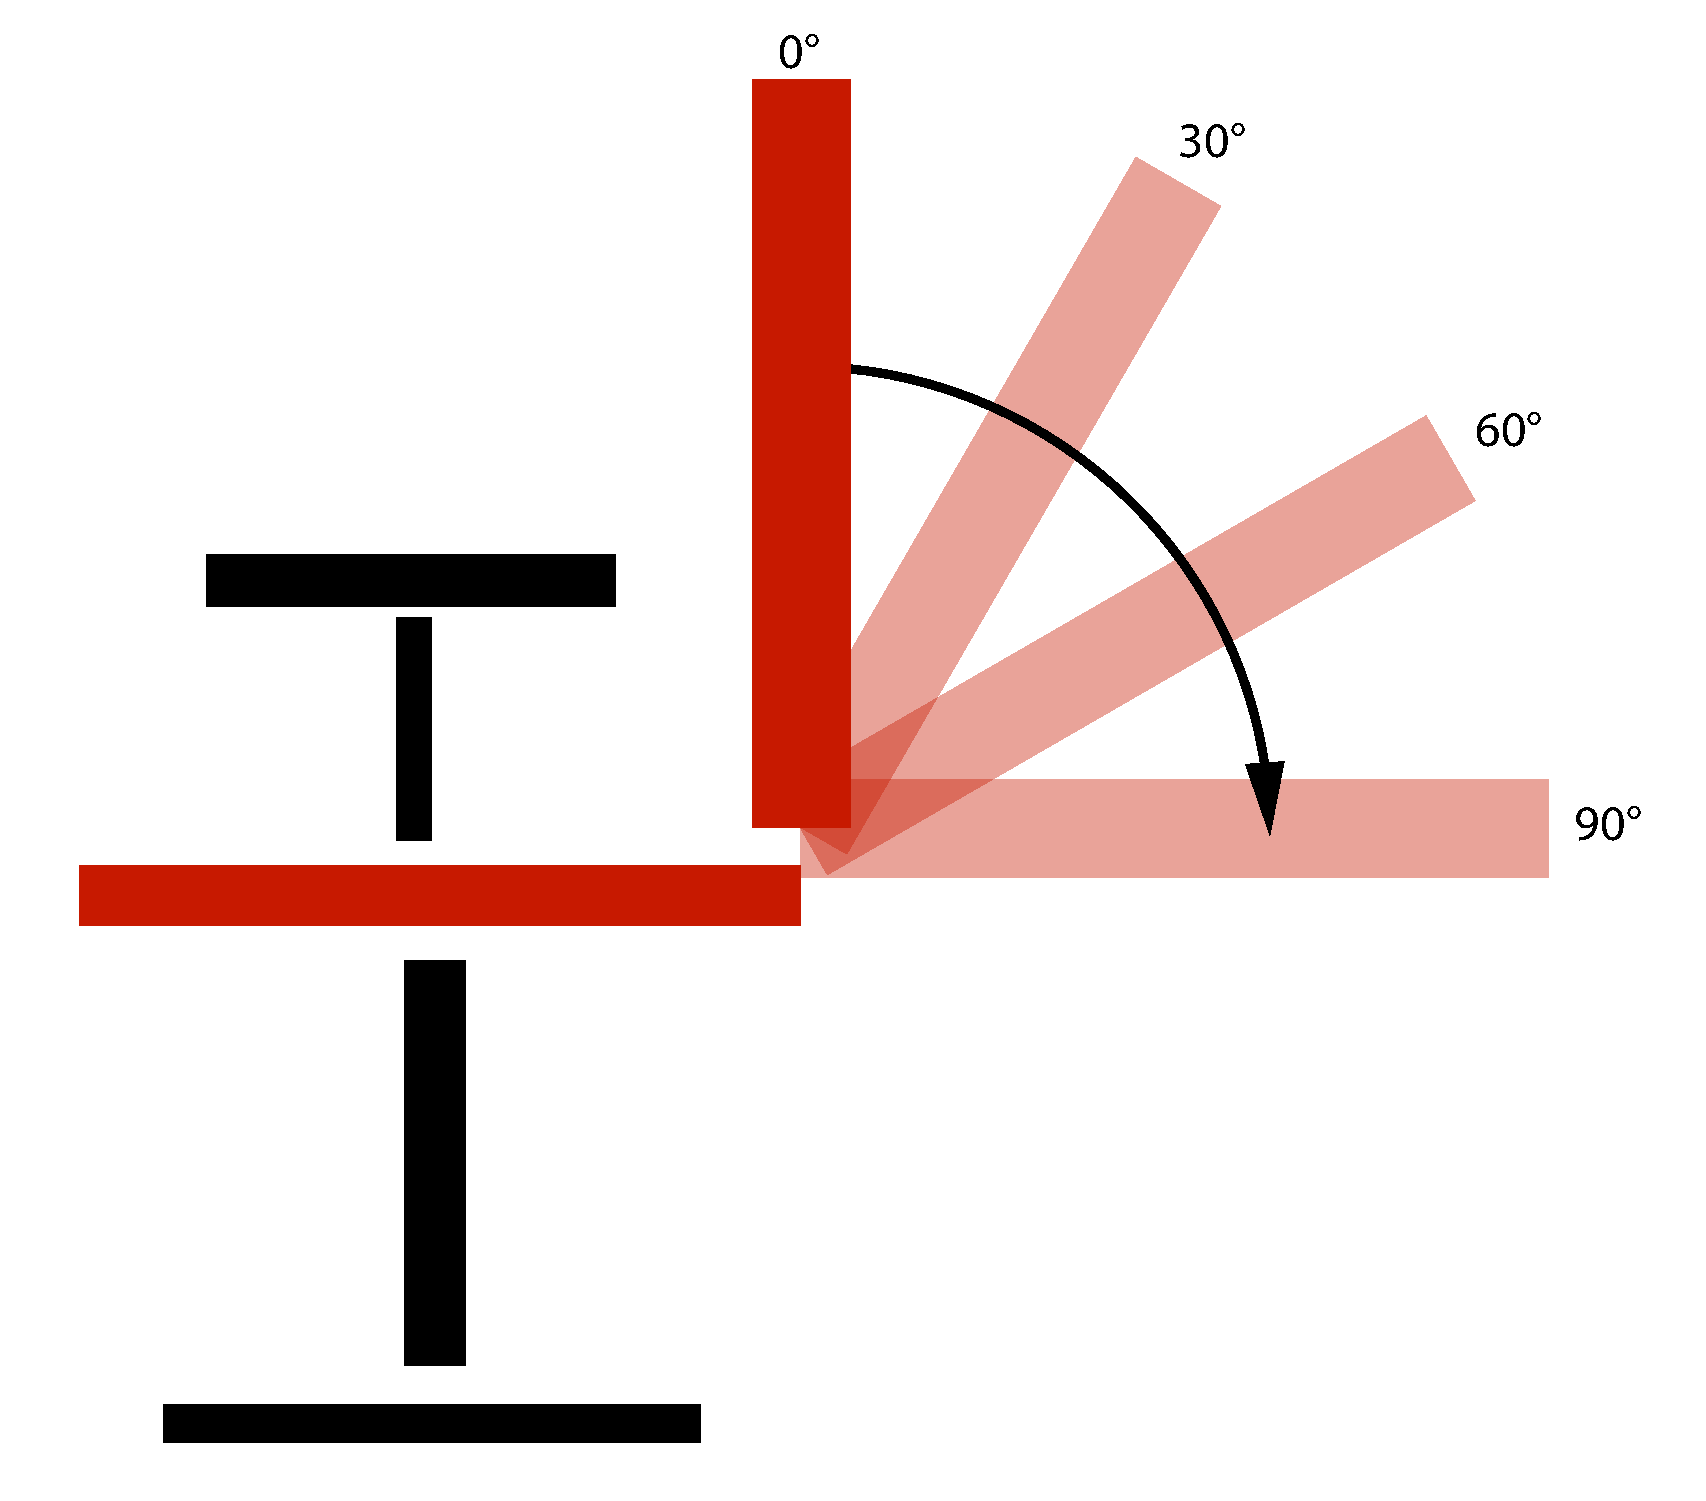
\includegraphics[width=0.75\textwidth]{./images/chair}
	\caption{Winkeleinstellungen vom verwendeten Stuhl in der Studie}
	\label{fig:chair_backrest}
\end{figure}

\subsection{Aufgabenergebnisse} %Fehler, Zeiten, pro Aufgaben
\todoLuc{Ergebnisse: Fehlerraten innerhalb der Aufgaben -> meint ihr (Luc, Sab) dass es hier eine bessere Art der Darstellung als ein Histogram gibt?}
\todoSab{Ergebnisse: Zeit für die Erledigung der Aufgaben -> meint ihr (Luc, Sab) dass es hier eine bessere Art der Darstellung als ein Histogram gibt?}
\todoTob{Ergebnisse: Dauer bis Probanden der 2. Studie den Ton abgeschalten haben}

Ein Hauptaspekt der Studie liegt auf der Aufgabenbewältigung und vor allem darauf, wie gut diese gelöst werden können unter den uns bekannten Umständen. 
\todoLuc{Aufgabenergebnisse Korrekturlesen und ergänzen bzw besser schreiben}

\subsubsection{Fehlerraten}

Für die erste Aufgabe gilt, dass ein Fehler dann als Fehler gewertet wird, wenn danach eine kleinere Zahl vorkommt. Eine ausgewählte Reihenfolge $3, 2, 1$ zählt also als 3 Fehler insgesamt, da $3 > 2 > 1$ (2 Fehler) sowie $2 > 1$ (1 Fehler). Auf diese Weise kommen auch 45 Fehler zustande; und zwar dann, wenn alle Zahlen falsch herum ausgewählt wurden. Dies entspricht der Summe von 1 bis 9.
Wie in Tabelle~\ref{fig:orderingMistakeHistogram} abzulesen, haben nur knapp 58\% der Studienteilnehmer überhaupt keine Fehler begangen. Häufig wurden vereinzelte Fehler gemacht, welche die Teilnehmer direkt beim Ausführen der Aufgabe bemerkten, was meist durch verbale oder physische Reaktionen deutlich wurde. 
Eine Fehlerzahl von 44 oder 45 wurde dann erreicht, wenn die Probanden gedacht haben, sie sollen genau anderherum sortieren, wie man uns im Nachhinein mitgeteilt hat.

\begin{figure}[H]
	\centering
	\includegraphics[width=0.75\textwidth]{./_StudyResults/orderingMisHist}
	\caption{Häufigkeit der Fehler in der ersten Aufgabe: Zahlenfolge. Darstellungsgenauigkeit: 1}
	\label{fig:orderingMistakeHistogram}
\end{figure}

\begin{table*}
	\caption{Vorkommnisse der Fehler in Aufgabe 1: Zahlenfolge.}~\label{tab:orderingMistakeNumbers}
	
	\setlength\tabcolsep{3pt}
	\renewcommand{\arraystretch}{1.4}% for the vertical padding
	\begin{tabularx}{\textwidth}{ | l | x | x | x | x | x | x | x | x | x | }
		\hline
		Anzahl Fehler & 0   & 1  & 2  & 4  & 6  & 13 & 17 & 44  & 45 \\ \hline\hline
		Häufigkeit 	  & 26  & 6  & 6  & 1  & 1  & 1  & 1  &  2  & 1  \\ \hline
	\end{tabularx}
\end{table*}

In Aufgabe 2 ist ein Fehler dann gegeben, wenn das ausgewählte Feld nicht dem gefordertem Feld entspricht, also ist das Maximum 10.
Von ca 73\% wurde diese Aufgabe komplett fehlerfrei gelöst.
Auch hier wurden Fehlerzahlen die 8 oder höher waren erzielt, da die Aufgabe so verstanden wurde, dass die Farbe in der das Wort geschrieben stand gewählt werden sollte.

\begin{figure}[H]
	\centering
	\includegraphics[width=0.75\textwidth]{./_StudyResults/matchingMisHist}
	\caption{Häufigkeit der Fehler in der Aufgabe 2: Stroop-Effekt. Darstellungsgenauigkeit: 1}
	\label{fig:matchingMistakeHistogram}
\end{figure}

\begin{table*}
	\caption{Vorkommnisse der Fehler in Aufgabe 2: Stroop-Effekt.}~\label{tab:matchingMistakeNumbers}
	
	\setlength\tabcolsep{3pt}
	\renewcommand{\arraystretch}{1.4}% for the vertical padding
	\begin{tabularx}{\textwidth}{ | l | x | x | x | x | x | x | x | }
		\hline
		Anzahl Fehler & 0   & 1  & 2  & 7  & 8  & 9 & 10 \\ \hline\hline
		Häufigkeit 	  & 33  & 4  & 2  & 2  & 1  & 2 & 1  \\ \hline
	\end{tabularx}
\end{table*}

In Aufgabe 3 zählt ein Fehler dann, wenn nicht die richtige Anzahl von den gegebenen Auswahlmöglichkeiten gewählt wurde. Die maximale Anzahl an Fehlern ist bei 3 Durchläufen also drei.
Von knapp 75\% wurde diese Aufgabe fehlerfrei gemeistert und kein Proband hat alle 3 Boxenzahlen falsch bestimmt. Die durchschnittliche Fehleranzahl beträgt 0.31, was im Anhang in Tabelle~\ref{tab:sc_results_counting} nachzulesen ist.

\begin{figure}[H]
	\centering
	\includegraphics[width=0.75\textwidth]{./_StudyResults/countingMisHist}
	\caption{Häufigkeit der Fehler in Aufgabe 3: Boxen zählen. Darstellungsgenauigkeit: 1}
	\label{fig:countingMistakeHistogram}
\end{figure}

\begin{table*}
	\caption{Vorkommnisse der Fehler in Aufgabe 3: Boxen zählen.}~\label{tab:countingMistakeNumbers}
	
	\setlength\tabcolsep{3pt}
	\renewcommand{\arraystretch}{1.4}% for the vertical padding
	\begin{tabularx}{\textwidth}{ | l | x | x | x | }
		\hline
		Anzahl Fehler & 0   & 1  & 2 \\ \hline\hline
		Häufigkeit 	  & 34  & 8  & 3 \\ \hline
	\end{tabularx}
\end{table*}

\subsubsection{Benötigte Zeit für die Aufgabenerledigung}
\todoTob{Hier Vielleicht Ergebnis der einzelnen Zeiten, also wie lange bis die erste Auswahl getroffen wurde; wie lange zwischen jeder Auswahl; gibt es Unterschiede wie schnell+falsch oder langsam+richtig oder auch schnell+richtig und langsam+falsch?}

Die jeweils gemessene Zeit erstreckt sich über den Start, der mit der Erklärung der Aufgabe gekennzeichnet wird, bis hin zum Ende der Zeitmessung, das den Abschluss der Aufgabe bedeutet.
Die Zeit, die für das Erledigen von Aufgabe 1 benötigt wurde, hat ihr Minimum bei 16.59 Sekunden. Die Anzahl der Teilnehmern die in einem Bereich von 2-Sekundenschritten, angefangen bei 15-17 Sekunden fertig geworden sind können in Abbildung~\ref{fig:orderingTimeHistogram} abgelesen werden. Die meistbenötigte Zeit 42.49 Sekunden, sowie ein Durchschnitt von 26.80 Sekunden können aus Tabelle~\ref{tab:times_results_ordering} entnommen werden.

\begin{figure}[H]
	\centering
	\includegraphics[width=0.75\textwidth]{./_StudyResults/orderingTimeHist}
	\caption{Histogramm der Zeit (ms) zur Erledigung von Aufgabe 1: Zahlenfolge. Genauigkeit: 2000ms}
	\label{fig:orderingTimeHistogram}
\end{figure}

Bei der zweiten Aufgabe gibt es eine größeren gemessenen Zeitbereich, was unter Anderem daran lag, dass die Probanden oft lang gebraucht haben die Aufgabenstellung zu lesen bzw. zu verstehen. Der schnellste Teilnehmer beendete die Aufgabe nach 13.87 Sekunden. Durchschnittlich haben die Probanden knapp 35 Sekunden zur Aufgabenbewältigung gebraucht. Das Maximum 83.31 Sekunden Bearbeitungszeit liegt in großem Abstand zum 'Zweitlangsamsten', welcher bei knapp unter 50 Sekunden liegt. Ein starker Häufungspunkt um die 20 Sekunden Marke kann man gut in Abbilung~\ref{fig:matchingTimeHistogram} erkennen.

\begin{figure}[H]
	\centering
	\includegraphics[width=0.75\textwidth]{./_StudyResults/matchingTimeHist}
	\caption{Histogramm der Zeit (ms) zur Erledigung von Aufgabe 2: Stroop-Effekt. Genauigkeit: 2000ms}
	\label{fig:matchingTimeHistogram}
\end{figure}

Zum Bearbeiten der Aufgabe wurde durchschnittlich 32.75 Sekunden gebraucht. 

\begin{figure}[H]
	\centering
	\includegraphics[width=0.75\textwidth]{./_StudyResults/countingTimeHist}
	\caption{Histogramm der Zeit (ms) zur Erledigung von Aufgabe 3: Boxen zählen. Genauigkeit: 2000ms}
	\label{fig:countingTimeHistogram}
\end{figure}

\subsubsection{Dauer des Wecker-Tons}
\begin{figure}[H]
	\centering
	\includegraphics[width=0.75\textwidth]{./_StudyResults/alarmDurationHist}
	\caption{Histogramm der Zeit (s), wie lange die Teilnehmer der Studie den Wecker-Ton laufen ließen. Genauigkeit: 500ms}
	\label{fig:countingTimeHistogram}
\end{figure}

\subsection{Selbsteinschätzungen, Fragebögen}\todoAll{subsection ggf umbennen}
%nur Vorschläge zur Gleiderung; hier sowas wie.. SAM, oder so..?

\todoTob{Ergebnisse: RSME Werte}
\todoTob{Ergebnisse: limesurvey zeug}
\todoTob{Ergebnisse: Kopfbewegungen}

\todoLuc{Abschnitt zu Ergebnisse von SAM schreiben}
Das Ausfüllen des SAM Fragebogen wurde einmal vor und einmal nach der Ruhephase verlangt. 

\begin{figure}[H]
	\centering
	\includegraphics[width=0.75\textwidth]{./_StudyResults/SAMpre}
	\caption{Self-Assessment Manikin Ergebnisse vor der Ruhephase}
	\label{fig:samPre}
\end{figure}%
\begin{figure}[H]
	\centering
	\includegraphics[width=0.75\textwidth]{./_StudyResults/SAMpost}
	\caption{Self-Assessment Manikin Ergebnisse nach der Ruhephase}
	\label{fig:samPost}
\end{figure}


Laut Befragung der Probanden im Anschluss an die Studie haben 20\% geschlafen, beziehungsweise mit den Teilnehmern, die fast geschlafen haben landet man bei 46,7\%. Ein geringer Prozentsatz hat meditiert und die anderen Nutzer gaben an nicht geschlafen zu haben, jedoch waren hier die meisten laut eigener Aussage trotzdem sehr entspannt. Genaue prozentuale Anteile können in Tabelle~\ref{tab:sleepstatus} entnommen werden. \todoTob{Ergebnisse: grafische Darstellung zu 'geschlafen'?}

Die empfundene Schlafdauer variiert in einem Zeitintervall zwischen 8 und 30 Minuten, wobei ein deutlicher Häufungspunkt bei der 15 Minuten Dauer anfällt und die 30 Minuten Angabe ein einzelner Ausreißer ist. Eine genaue Auflistung der Zeitangaben kann in Tabelle~\ref{tab:sleepduration} eingesehen werden.
\todoTob{Ergebnisse: Empfundene Dauer der Ruhephase}
